\documentclass[11pt]{article}
\usepackage[utf8]{inputenc}
\usepackage{graphicx}
\usepackage{float}
\usepackage{amsmath}
\usepackage[natbibapa]{apacite}
\usepackage[table]{xcolor}
\usepackage{setspace}
\onehalfspacing
\usepackage{subcaption}
\usepackage[numbers]{natbib}
\usepackage[skip=0.5\baselineskip]{caption} 
\usepackage[left=2cm,right=2cm,top=1.5cm,bottom=1.5cm]{geometry}

\title{Can ML Beat Baseline Models? Forecasting Methods \\ for Indian REITs and Real Estate Equities}
\author{
    Borishan Ghosh\textsuperscript{1}, Sanjana Dutta\textsuperscript{2} \\
    \small \textsuperscript{1}Department of Physics, Hansraj College, University of Delhi, \texttt{borishan.gh@gmail.com} \\
    \small \textsuperscript{2}Department of Economics, Jesus and Mary College, University of Delhi, \texttt{sanjana.dutta1306@gmail.com}
}
\date{\vspace{-2ex}}

\begin{document}

\maketitle

% Abstract
\begin{abstract}
    \noindent Predicting stock prices in markets such as REITs and real estate equities is a popular challenge for time series forecasting methods. The inherent volatility and self-correcting nature of these markets raise fundamental questions about the applicability of statistical learning methods. This study challenges the notion of prediction of stock movement being a time series problem in view of the Efficient Market Hypothesis. \\
    We compare tree-based models (XGBoost, Random Forests), LSTMs, transformers, and other popular approaches against baseline models and linear regression techniques that fit linear and polynomial curves to past trends. Employing feature engineering and hyperparameter tuning, nonlinear relationships and associated stock trends is learned. Models are evaluated using walk-forward validation on Indian REIT and real estate equity data from 2015-2023. Performance is analyzed using financial metrics (beta, volume, rolling volatility) and fundamental indicators (profit after tax, return on equity, price-earning ratios) with RMSE, MAE, and directional accuracy as key metrics.
\end{abstract}

\section{Introduction}
\label{sec:introduction}
REITs (Real Estate Investment Trusts) and real estate stocks offer ways to invest in the property market, but they function differently. REITs are companies that own or finance income-producing real estate across various sectors like commercial, residential, and industrial. Structured to distribute a significant portion of their taxable income as dividends (often above 90\%), REITs provide investors regular income.

\begin{figure}[htbp]
    \centering
    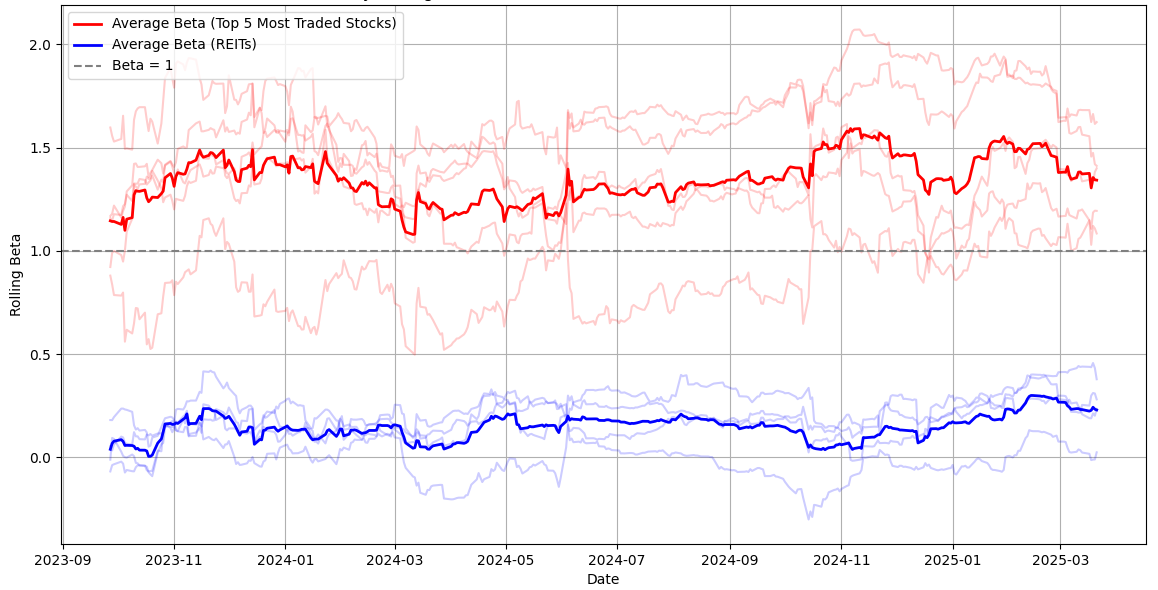
\includegraphics[width=0.7\textwidth]{figures/rolling_beta.png}
    \caption{90 day Rolling Beta of Stocks vs. REITs relative to \^NSEI}
    \label{fig:sample}
\end{figure}

Real estate stocks, on the other hand, represent ownership in companies involved in property development, management, or sales. Unlike REITs, these companies may retain more earnings for reinvestment and growth, and their value is tied to project success and market conditions rather than solely rental income.


\section{Methodology}
\label{sec:methodology}

\subsection{Data Description}
Closing prices of REITs and real estate equities are collected from Yahoo Finance over the data range 01-01-2005 till 01-04-2025, a train-test split is made at 01-01-2023. Moving window subsets of past 60 closing prices are used as features with the target variable being the closing price of the next day. Additionally indicators such as RSI, and competitor features are also incorporated.\cite{1}

\begin{figure}[htbp]
    \centering
    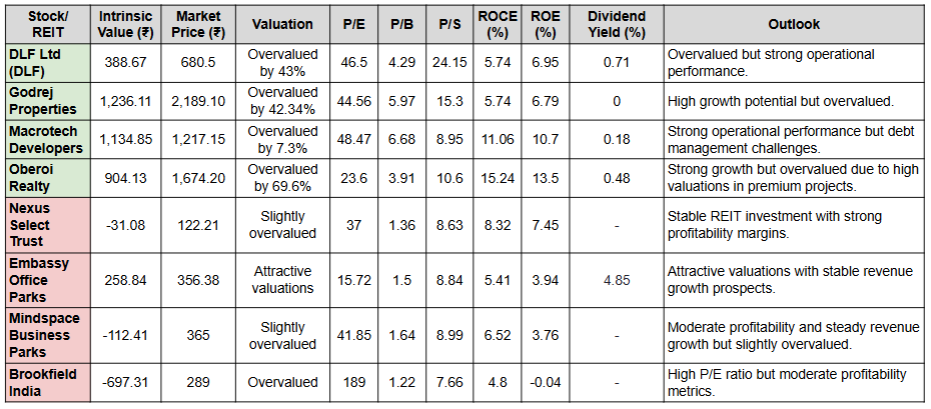
\includegraphics[width=0.9\textwidth]{figures/markt_summary.png}
    \caption{Fundamental analysis of stocks can be incorporated as model context}
    \label{fig:sample}
\end{figure}

Financial ratios such as P/E, P/B, and P/S, show valuation relative to earnings, book value and sales respectively. Profitability metrics such as ROCE and ROE reveal how effectively a company generates profits from its capital and equity. The debt-to-equity ratio indicates financial leverage, while the dividend yield shows the return on investment through dividends.\cite{2}
Using these financial metrics and comparing against industry peers and historical performance, analysts can assess a stock’s potential and hence make informed investment decisions.\cite{6}


\subsection{Model Specifications}

\textit{Baseline Models} :  The strategies used as a baseline are \texttt{last\_price} (returns the closing price of previous day), \texttt{mean} (returns the mean closing price of last 7 days), \texttt{linear} (fits a line to last 7 days of prices), \texttt{quadratic} (fits a quadratic curve to last 7 days of prices)

\vspace{1em}

\textit{Long Short-Term Memory network} : Three \texttt{LSTM} layers with 128, 64, and 32 units, using tanh activation. Dropout layers (rate=0.3) added to prevent overfitting after each LSTM layer for regularization. Final dense layer uses ReLU activation for output transformation. Model is trained using walk-forward validation with 30 epochs and early stopping.

\vspace{1em}

\textit{Tree-based Models} : \texttt{RandomForestRegressor} over 200 decision trees with max depth of 20. \texttt{XGBRegressor} over 200 boosted trees with max depth of 6, learning rate of 0.1 with subsampling and L2 regularization. Models are further subjected to hyperparameter tuning through grid search. 

\vspace{1em}

\textit{Ridge Regression}: We use \texttt{Ridge} regression with L2 (\(\alpha = 1\)) regularization with standardized features before fitting. This serves as a linear benchmark for the above nonlinear models.

\section{Key Findings}
\label{sec:keyfindings}

\subsection{Long Short-Term Memory Networks}

\begin{figure}[h!]
    \centering
    \begin{tabular}{cc}
        % Row 1
        \begin{subfigure}[b]{0.48\textwidth}
            \centering
            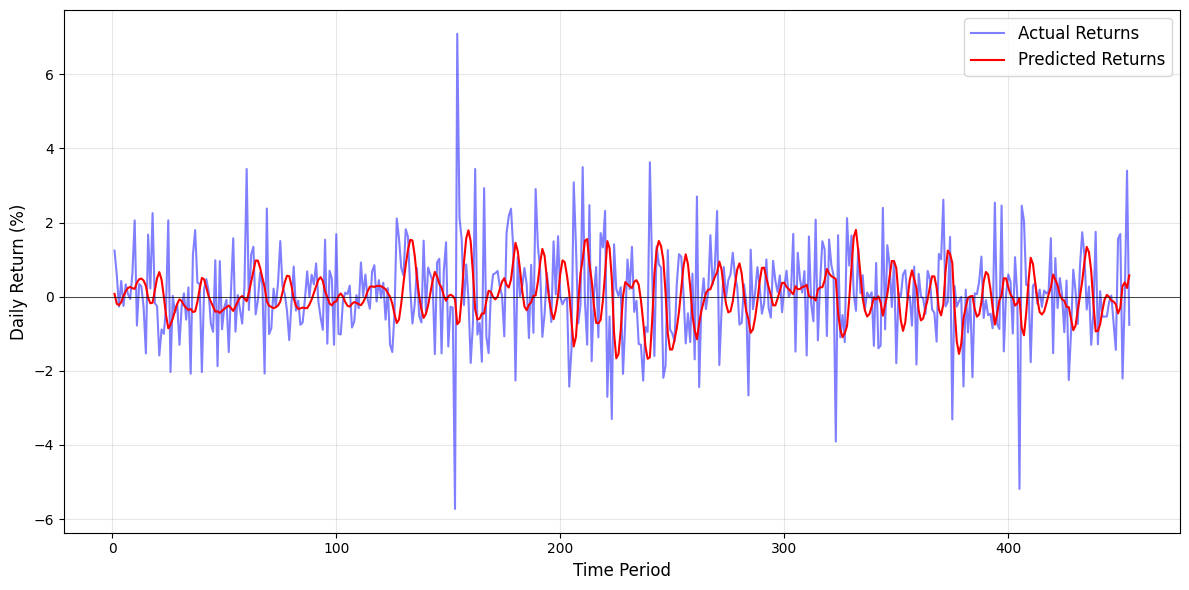
\includegraphics[width=\linewidth]{figures/lstm/lstm_embassy.png}
            \caption{daily returns for EMBASSY.BO (50 epochs)}
            \label{fig:1a}
        \end{subfigure} &
        \begin{subfigure}[b]{0.48\textwidth}
            \centering
            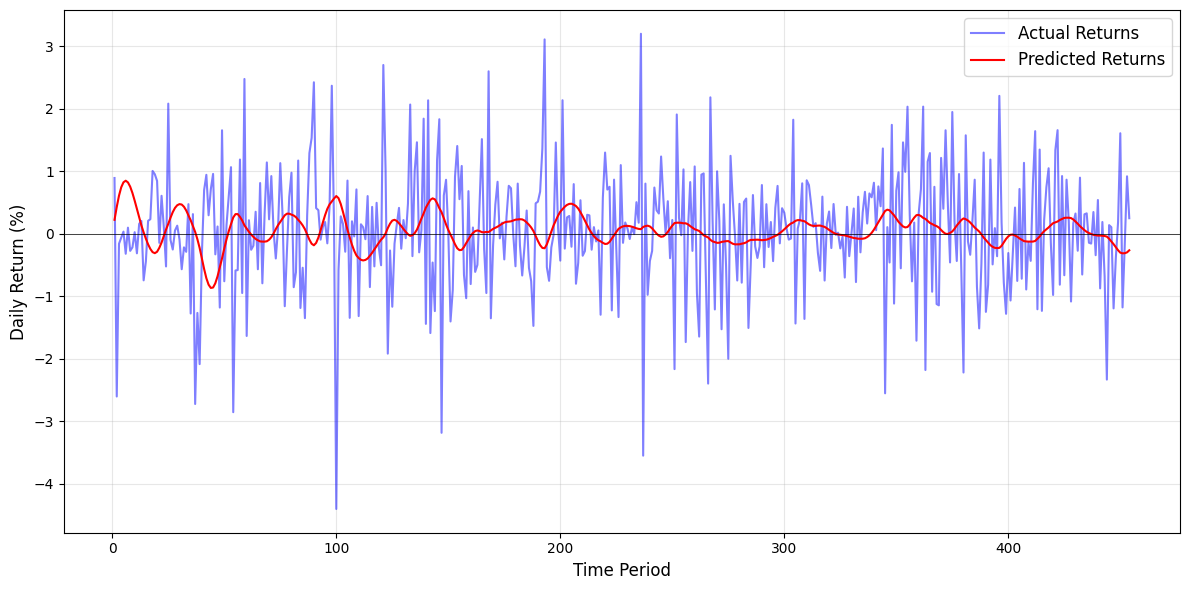
\includegraphics[width=\linewidth]{figures/lstm/lstm_mindspace_epoch30.png}
            \caption{daily returns for EMBASSY.BO (30 epochs)}
            \label{fig:1b}
        \end{subfigure} \\
    \end{tabular}
    \label{fig:4x2grid}
    \caption{LSTM trained for different epochs don't show significant improvement}
\end{figure}

The proponents of LSTM as a candidate model for stock forecast often emphasize its performance over standard metrics such as Mean Absolute Percentage Error(MAPE) over Close prices. However we note that LSTM consistently scores lower than baseline at directional accuracy scores.\cite{3}

Looking at daily returns reveals the inadequacy of the neural network at capturing the stochastic nature of the trend (above). Training over longer epochs makes the predicted trend more granular without any substantial increase in accuracy.


\subsection{Tree Based Models}

\begin{figure}[h!]
    \centering
    \begin{tabular}{cc}
        % Row 1
        \begin{subfigure}[b]{0.48\textwidth}
            \centering
            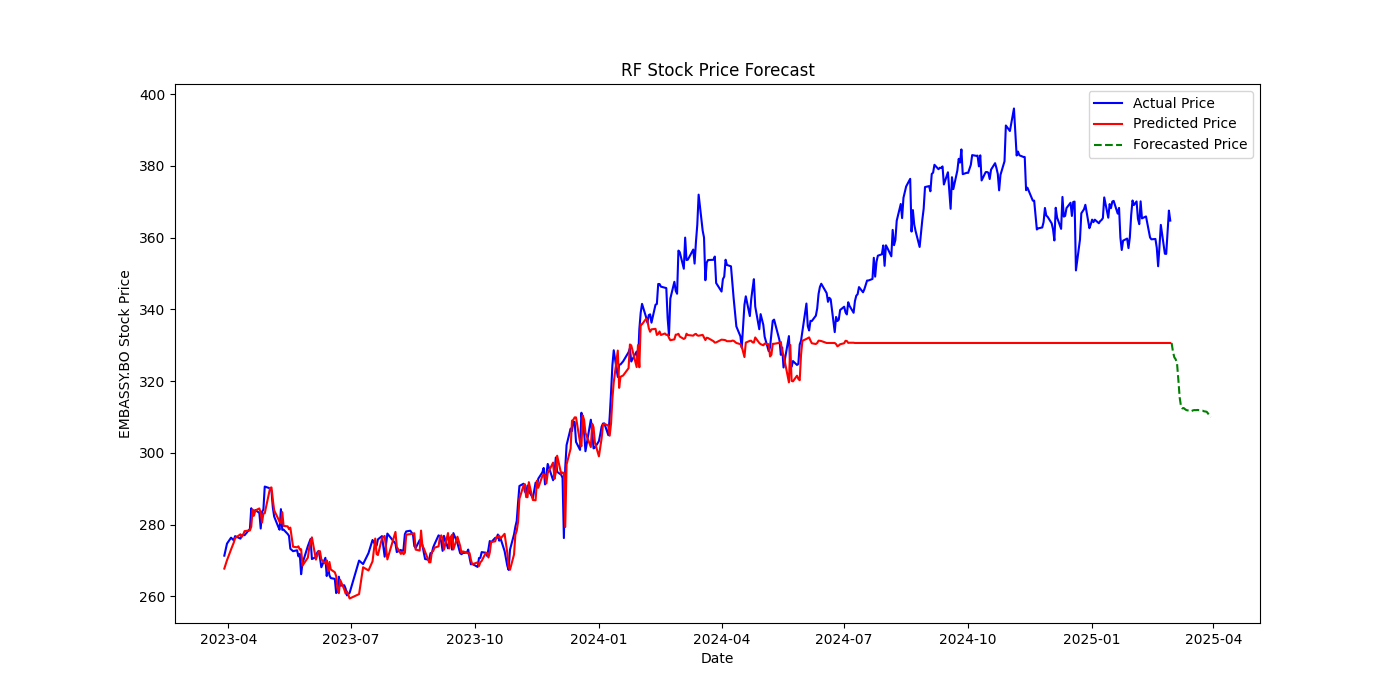
\includegraphics[width=\linewidth]{figures/rf/EMBASSY_predict.png}
            \caption{RFRegressor over EMBASSY.BO trend}
            \label{fig:1a}
        \end{subfigure} &
        \begin{subfigure}[b]{0.48\textwidth}
            \centering
            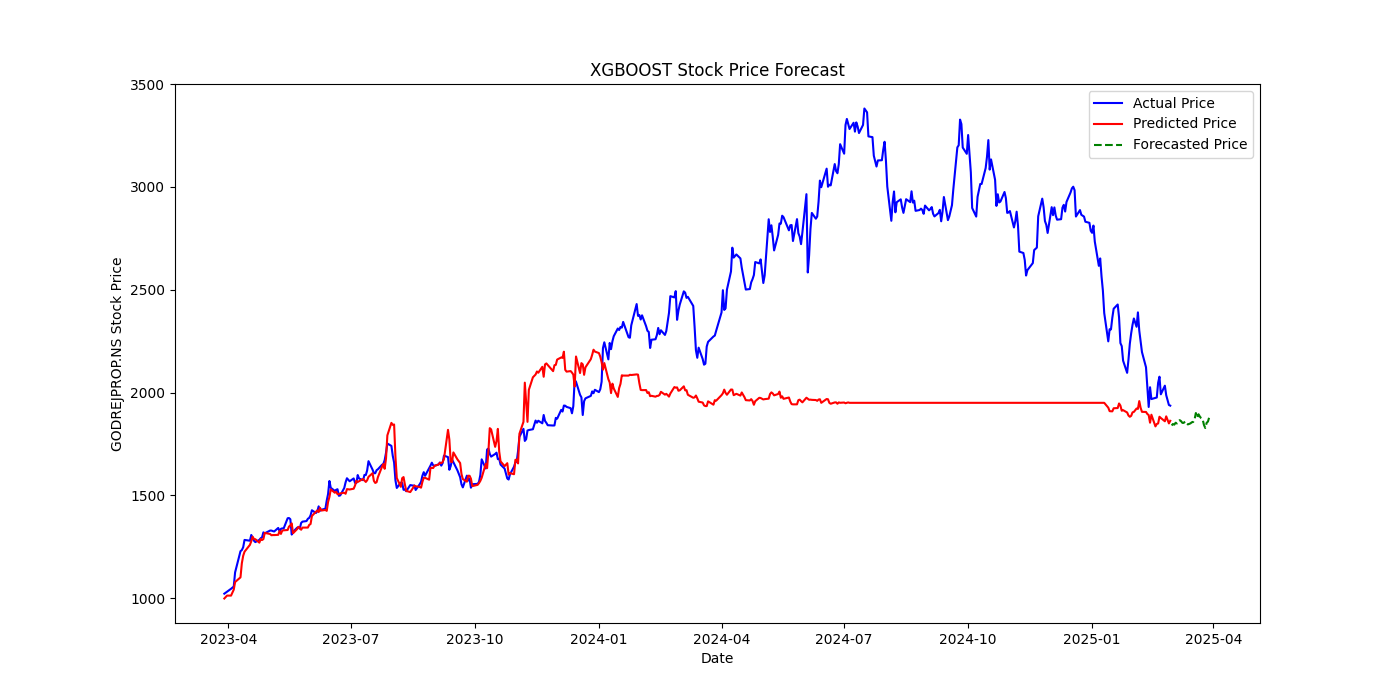
\includegraphics[width=\linewidth]{figures/xgboost/GODREJPROP_predict.png}
            \caption{XGBoost over GODREJPROP.NS trend}
            \label{fig:1b}
        \end{subfigure} \\
    \end{tabular}
    \caption{Tree based models are mean-reverting by nature}
    \label{fig:4x2grid}
\end{figure}

Tree based models in their design fail to account for temporal awareness, treating each input window independently without memory of past sequences. \texttt{RFRegressor} / \texttt{XGBRegressor} interpolate well at short initial stretches but fail at extrapolation, reverting to mean predictions when faced with unseen trends.\cite{4}

\begin{figure}[h!]
    \centering
    \begin{tabular}{cc}
        % Row 1
        \begin{subfigure}[b]{0.48\textwidth}
            \centering
            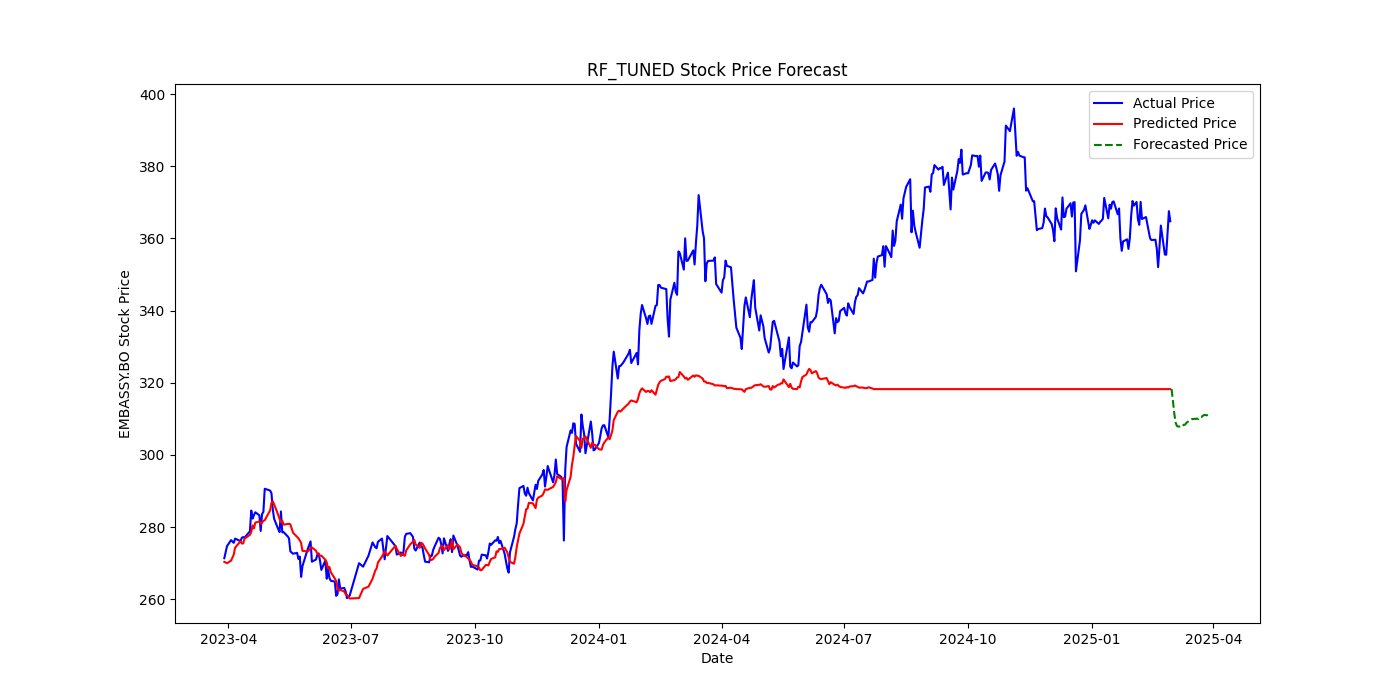
\includegraphics[width=\linewidth]{figures/rf_tuned/EMBASSY_predict.png}
            \caption{RF with hyperparameter tuning over EMBASSY.BO trend}
            \label{fig:1a}
        \end{subfigure} &
        \begin{subfigure}[b]{0.48\textwidth}
            \centering
            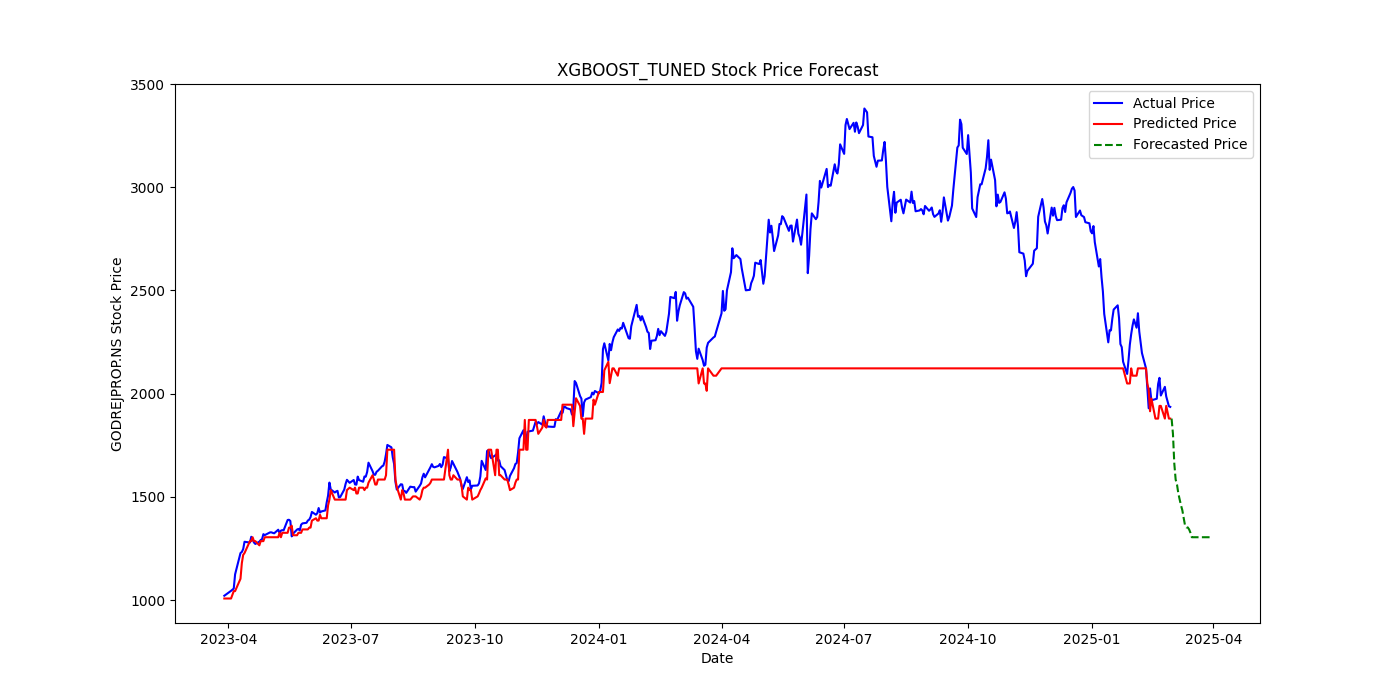
\includegraphics[width=\linewidth]{figures/xgboost_tuned/GODREJPROP_predict.png}
            \caption{XGBoost with hyperparameter tuning over GODREJPROP.NS trend}
            \label{fig:1b}
        \end{subfigure} \\
    \end{tabular}
    \caption{Hyperparameter tuning fail to correct for bad extrapolation}
    \label{fig:4x2grid}
\end{figure}

In effect, these models will never predict a price that it hasn't encountered before. Such behaviour is not correct even after extensive hyperparameter tuning. While tuning may improve fit (e.g., adjusting max\_depth or n\_estimators), it doesn’t improve the flaw in trend extrapolation. Trees are constrained by their split logic, unable to model unseen sequential patterns. \cite{5}


\section{Conclusion}
\label{sec:conclusion}

\begin{figure}[htbp]
    \centering
    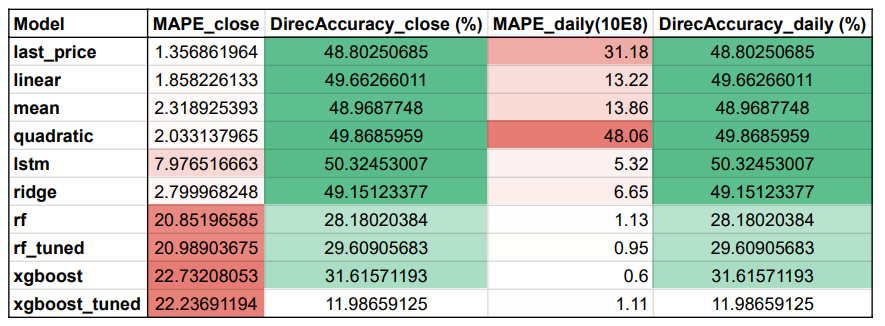
\includegraphics[width=0.8\textwidth]{figures/summary.png}
    \caption{Summary statistics of ML vs. Baseline models}
    \label{fig:sample}
\end{figure}

The most performant model analyzed is the Ridge regressor, which is at best a linear benchmark. ML models that utilize neural nets or train to capture non-linear trends are marginally suited to predict the general direction of the daily trend. However the successes over time are not statistically significant given their sophistication.
\newpage
\begin{figure}[htbp]
    \centering
    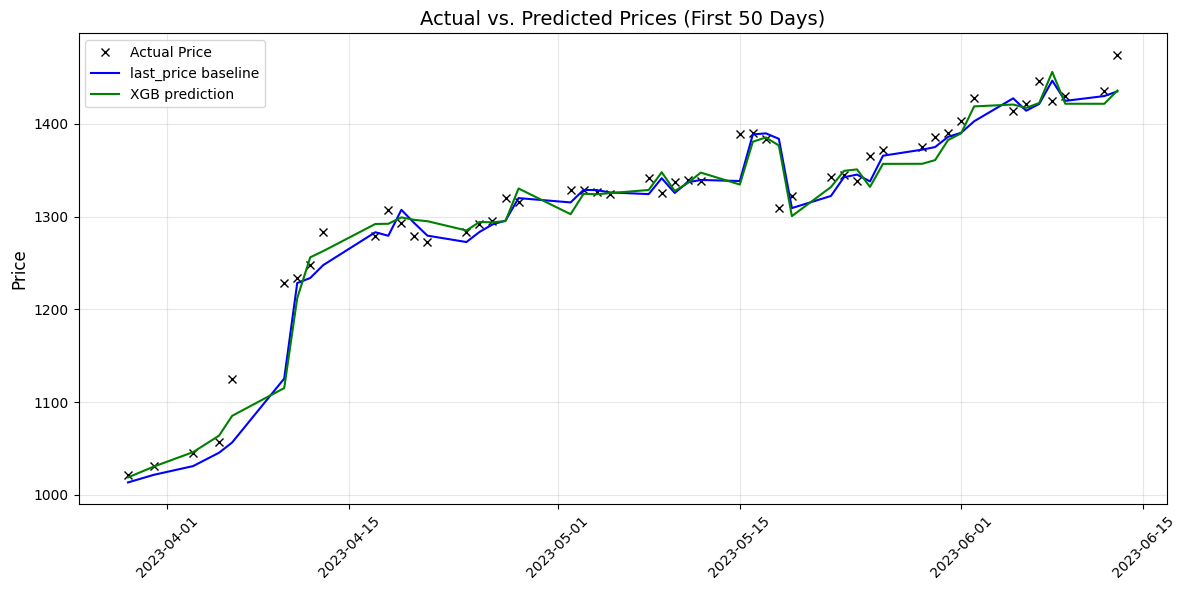
\includegraphics[width=0.8\textwidth]{figures/cgbfail.png}
    \caption{"Predicted" trends tend to trail the $\texttt{last\_price}$
    baseline instead of actual price.}
    \label{fig:sample}
\end{figure}

These models remain highly prone to overfitting and/or dataset poisoning and most require careful training and feature engineering. This study provides empirical evidence that for most purposes out-of-the-box ML models do not outperform baseline at predicting the movement of the market.

\begin{thebibliography}{9}

[1] \bibitem{1} 
Lindenthal, T., \& Leow, K. S. (2024). Enhancing real estate investment trust return forecasts using machine learning. \textit{Real Estate Economics}. Advance online publication. https://doi.org/10.2139/ssrn.4923052\\ \vspace{.5em}

[2] \bibitem{2} 
Foster, G. (2002). \textit{Financial statement analysis} (2nd ed.). Pearson Education.\\ \vspace{.5em}

[3] \bibitem{3} 
Kumar, R., \& Sharma, A. (2020). Optimizing LSTM for time series prediction in Indian stock market. \textit{Procedia Computer Science, 167}, 2091-2100. https://doi.org/10.1016/j.procs.2020.03.257\\ \vspace{.5em}

[4] \bibitem{4} 
Patel, J., Shah, S., Thakkar, P., \& Kotecha, K. (2018). Predicting the direction of stock market prices using tree-based classifiers. \textit{North American Journal of Economics and Finance, 45}, 146-159. https://doi.org/10.1016/j.najef.2018.06.013\\ \vspace{.5em}

[5] \bibitem{5} 
Zhang, Y., \& Li, X. (2020). Evaluation of tree-based ensemble machine learning models in predicting stock price direction of movement. \textit{Information, 11}(6), 332. https://doi.org/10.3390/info11060332\\ \vspace{.5em}

[6] \bibitem{6} 
Chen, W., \& Zhang, H. (2022). Machine learning for stock prediction based on fundamental analysis. \textit{arXiv}. https://doi.org/10.48550/arXiv.2202.05702

\end{thebibliography}

\newpage
\section{Appendix}

\begin{figure}[h!]
    \centering
    \begin{tabular}{cc}
        % Row 1
        \begin{subfigure}[b]{0.48\textwidth}
            \centering
            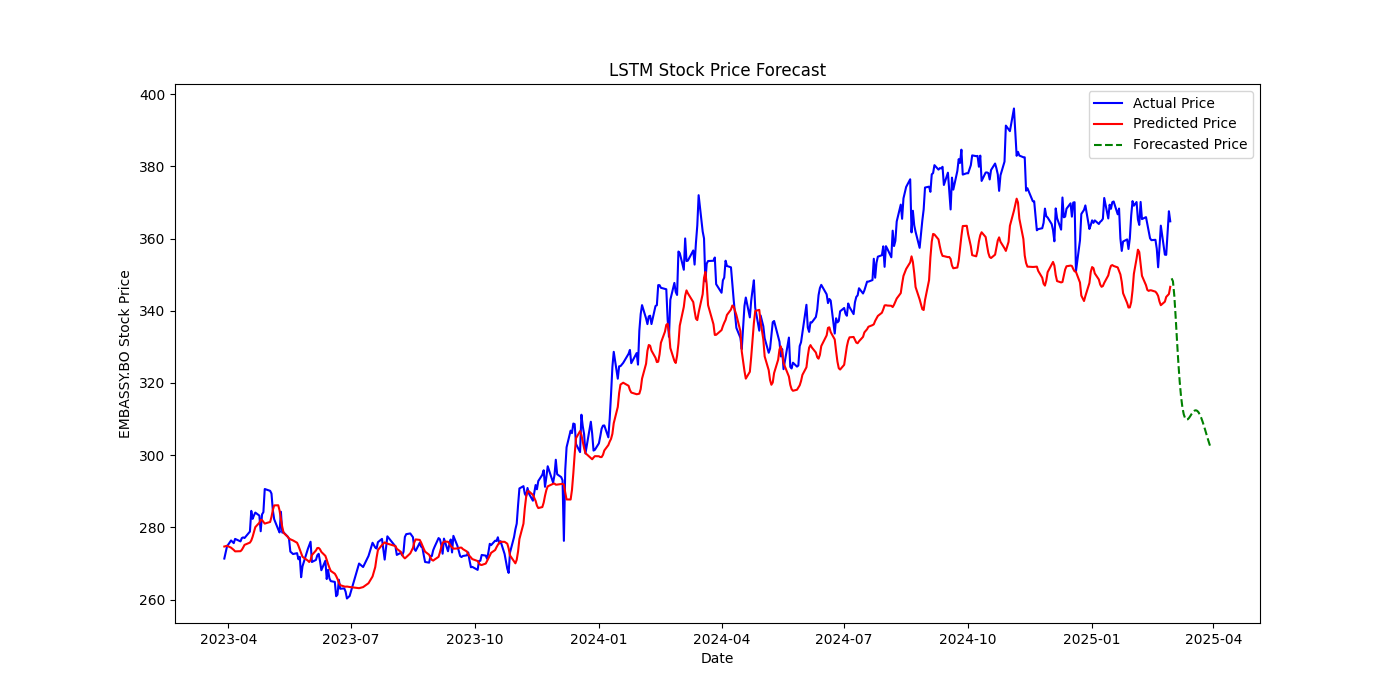
\includegraphics[width=\linewidth]{figures/lstm/EMBASSY_predict.png}
            \caption{LSTM over EMBASSY.BO trend}
            \label{fig:1a}
        \end{subfigure} &
        \begin{subfigure}[b]{0.48\textwidth}
            \centering
            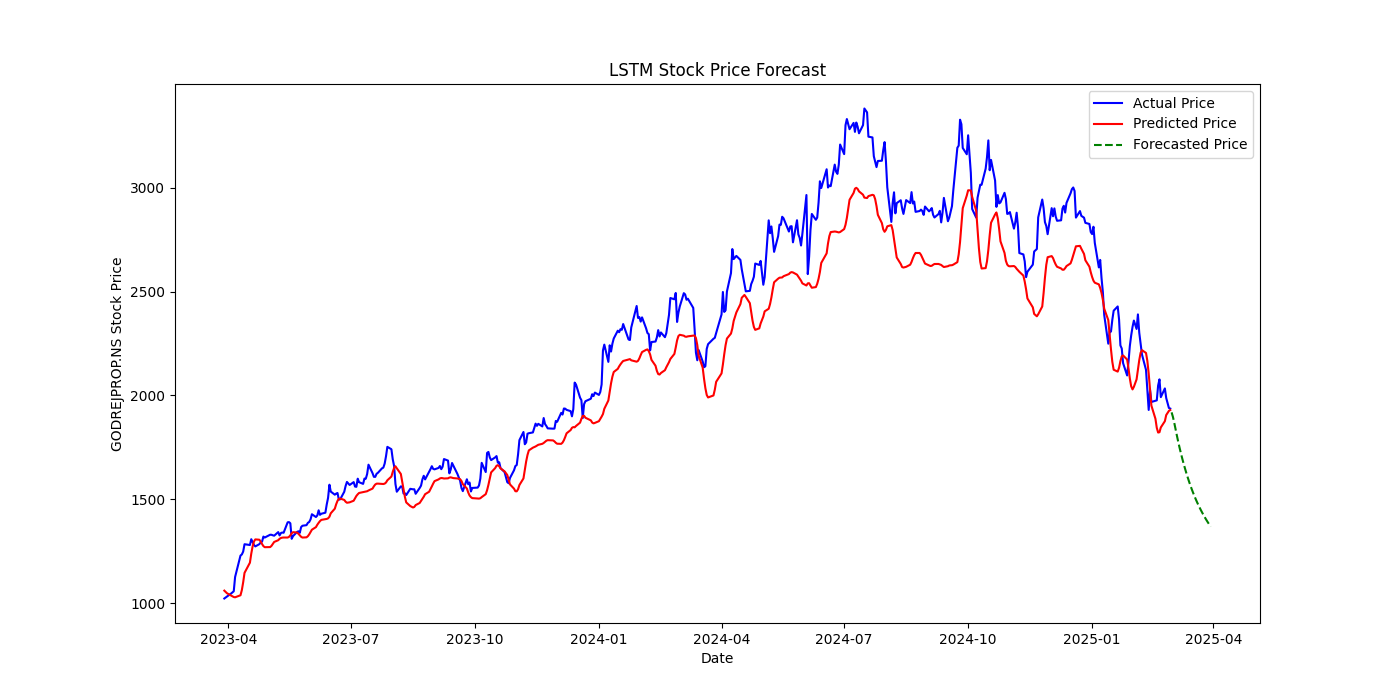
\includegraphics[width=\linewidth]{figures/lstm/GODREJPROP_predict.png}
            \caption{LSTM over GODREJPROP.NS trend}
            \label{fig:1b}
        \end{subfigure} \\
        
        \begin{subfigure}[b]{0.48\textwidth}
            \centering
            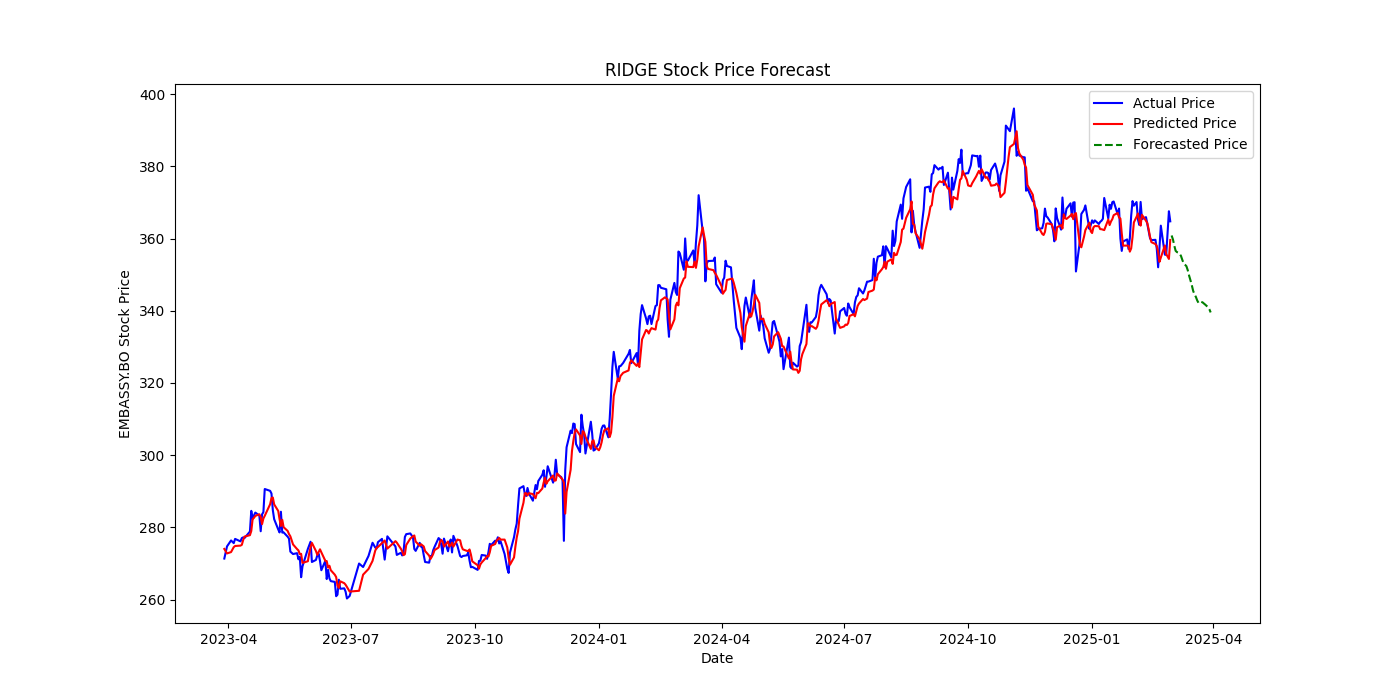
\includegraphics[width=\linewidth]{figures/ridge/EMBASSY_predict.png}
            \caption{Ridge over EMBASSY.BO trend}
            \label{fig:1a}
        \end{subfigure} &
        \begin{subfigure}[b]{0.48\textwidth}
            \centering
            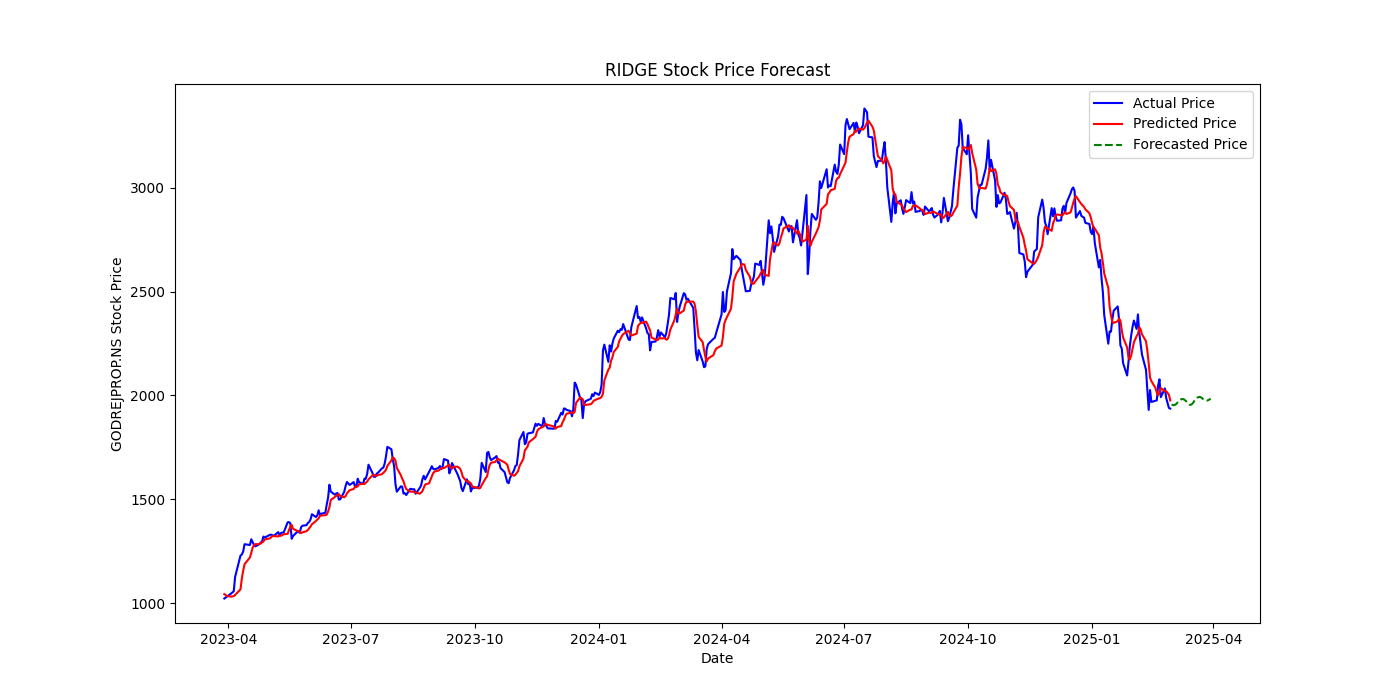
\includegraphics[width=\linewidth]{figures/ridge/GODREJPROP_predict.png}
            \caption{Ridge over GODREJPROP.NS trend}
            \label{fig:1b}
        \end{subfigure} \\
        
        \begin{subfigure}[b]{0.48\textwidth}
            \centering
            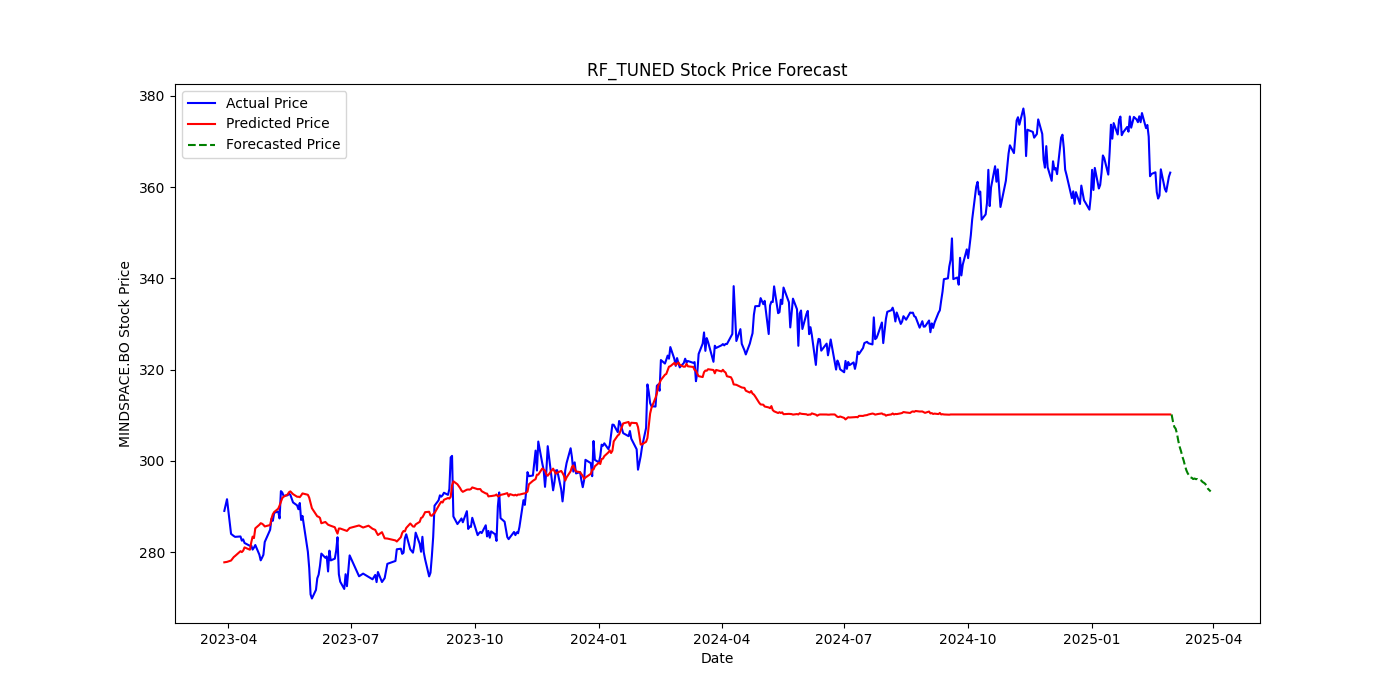
\includegraphics[width=\linewidth]{figures/rf_tuned/MINDSPACE_predict.png}
            \caption{RFRegressor over MINDSPACE.BO trend}
            \label{fig:1a}
        \end{subfigure} &
        \begin{subfigure}[b]{0.48\textwidth}
            \centering
            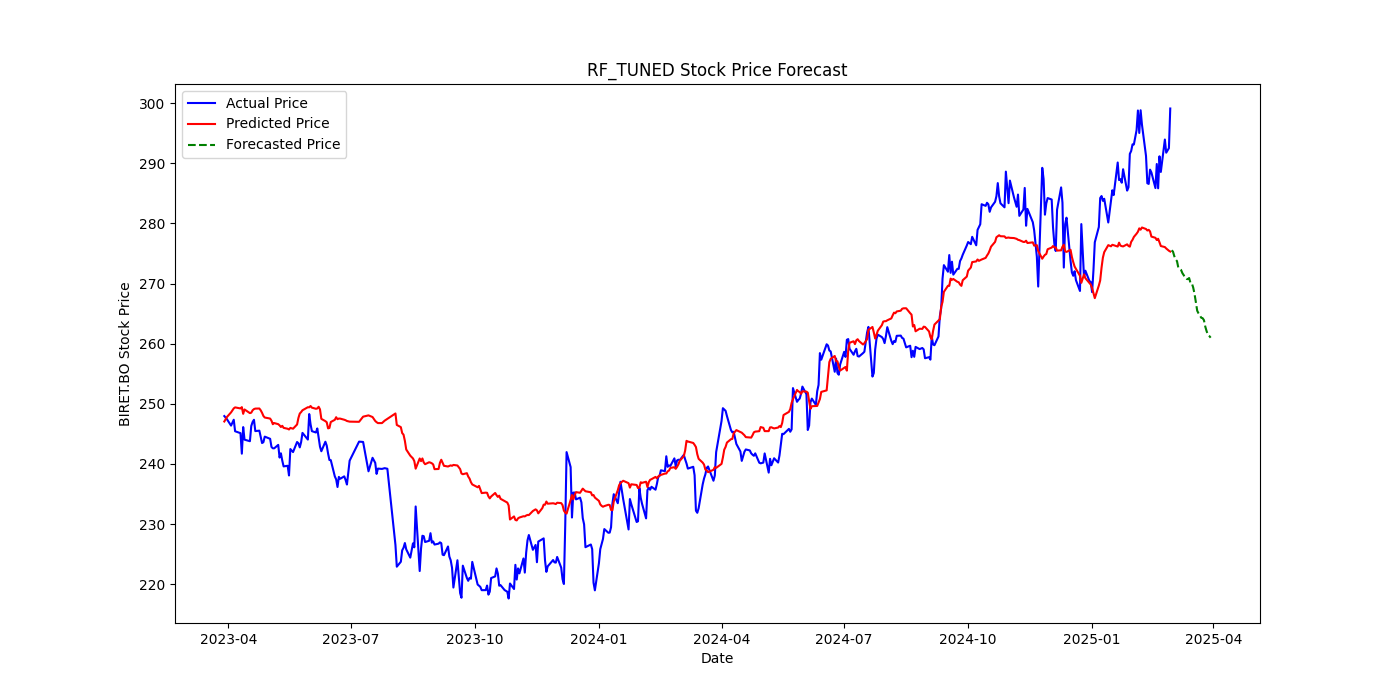
\includegraphics[width=\linewidth]{figures/rf_tuned/BIRET_predict.png}
            \caption{RFRegressor over BIRET.BO trend}
            \label{fig:1b}
        \end{subfigure} \\
    \end{tabular}
    \caption{Additional graphs}
    \label{fig:4x2grid}
\end{figure}

\end{document}